\section{Evaluation}

The present section aims at evaluating the behavior of the \schim on
the target platform, it overhead and benefits.  First, in subsection
\ref{subsection:considered-architecture}, we review our experimental
setup. Thereafter, we assess the overhead introduced by the \schim in
Section~\ref{subsec:platform-capabilities-and-performance-degradation}. In
Section~\ref{subsec:internal-behaviour-of-schim}, an in-depth analysis
of the \schim behaviour is presented. Finally, a demonstration of the
memory isolation enabled by the \schim using real-world benchmarks is
provided in Section~\ref{subsec:isolation}.
  

\subsection{Experimental Setup}
\label{subsection:considered-architecture}
The \schim has been evaluated using synthetic benchmarks (or
\emph{Memory Bombs}), real benchmarks selected from the San Diego
Vision Benchmark Suite (SD-VBS)~\cite{SD-VBS} and a combinations of
the two. Specifically, the 7 most memory-intensive benchmarks have
been selected, i.e. \emph{stitch}, \emph{texture synthesis},
\emph{disparity}, \emph{tracking}, \emph{localization}, \emph{mser}
and \emph{sift}. For all our runs we have considered the VGA input
size (640$\times$480 pixels). When running any benchmark, we use the
cache coloring mechanism provided by Jailhouse to partition the LLC
evenly amongst the cores and to prevent our measurements to be
affected by inter-core cache line eviction. As a result, each
benchmark operates on 1/4 of the total cache space---256~KB.

%  \todo[inline]{RM: this part is a bit redundant with the implementation section. We can remove this seciton and only keep the description of the routes we are gonna test. See above}
%    The COTS platform used for the following set of experiments, the Xilinx ZCU102 development board, features four cores which, with the LLC, composed the cores cluster. While the \schim can be configured to handle many more masters, in the present set of experiments, only the cores composing this cluster competes for main memory access. Consequently, the \schim module has been configured with four queues (one for each master) as shown in Figure \ref{fig:MemorEDF_module_schema}. Following the discussion in section \ref{sec:pl-to-ps-feedback}, \schim has been configured with two slave ports. Finally, the frequency of the PL side has been pushed to 250~MHz.

%    \todo[inline]{RM: The paragraph below to go into experimental setup}
To evaluate the capabilities of the \schim, three memory routes for
the traffic generated by the cores are compared. The first two serve
as baselines, whereas, the last one is the one under analysis and
involves the \schim module.  The first path consists in the cores
directly accessing the main memory. As illustrated in
\fig{fig:PS-PL-diagram}, the traffic simply goes through the
\emph{Main Interconnect} before arriving at the DDR controller. This
path is referred to as the \emph{normal route}. In the second path,
traffic is routed through the PL but without being subject to
scheduling. In this case, a simple one-to-one connection between one
of the HPM ports and the HPS port is programmed in the PL. No other
manipulation on the traversing memory transactions is performed inside
the PL; we refer to this case as the \emph{simple loop-back}. Finally,
we consider a third case where the \schim module is deployed and in
use to schedule memory traffic generated by the CPUs in the PL. Cores
0 and 1 target HPM1 aperture, while cores 2 and 3 target HPM2. In our
analysis, \schim is used in all the available modes, i.e., FP, TDMA
and TS.

\subsection{Platform Capabilities and performance degradation}
\label{subsec:platform-capabilities-and-performance-degradation}
Intuitively and as discussed in~\cite{PLIM20}, redirecting the traffic
coming from the cores to the PL side incurs a performance hit. In
fact, the PL operates at a lower frequency compared to the PS. As
such, larger memory latency and a smaller throughput should be
expected when routing memory traffic through the PL. On the other
hand, by redirecting and scheduling traffic in the PL, we can achieve
higher system predictability.  In order to weight up the pros and the
cons of these two orthogonal objectives, we have computed the
throughput of one \emph{core under analysis}, here core 0 (noted
$C_{0}$), for each of the aforementioned paths under all the possible
levels of contention. The result of this experiment is display in
\fig{fig:bandwidth_comparison}.
    
From \fig{fig:bandwidth_comparison}, one can observe that in general,
the throughput experienced by the core under analysis (i.e., $C_{0}$)
is high and that, regardless of the contention level on the normal
route, the bandwidth remains high. As mentioned earlier, redirecting
the cores' traffic through the PL side has a cost. In fact, in the
case with no contention (the left-most bar cluster), the bandwidth
experienced by $C_{0}$ when going through the simple loop-back, is
reduced by around 75\% compared to the normal route.  Looking at the
left-most bar cluster, one can also observe the overhead introduced by
having the presence of the \schim on the memory loop-back. The
additional drop in bandwidth is approximately 185~MBps.  While the
throughput is larger in the case of the \emph{simple loop-back}, it
also drops linearly as soon as the contention level increases.  On the
other hand, the \schim manages to preserve the same bandwidth, with
negligible interference being observed in the most challenging
scenario (the right-most bar cluster). In other words, the \schim
guarantees performance isolation between the cores with respect to the
bus usage.
     
\begin{figure}
  \centering
  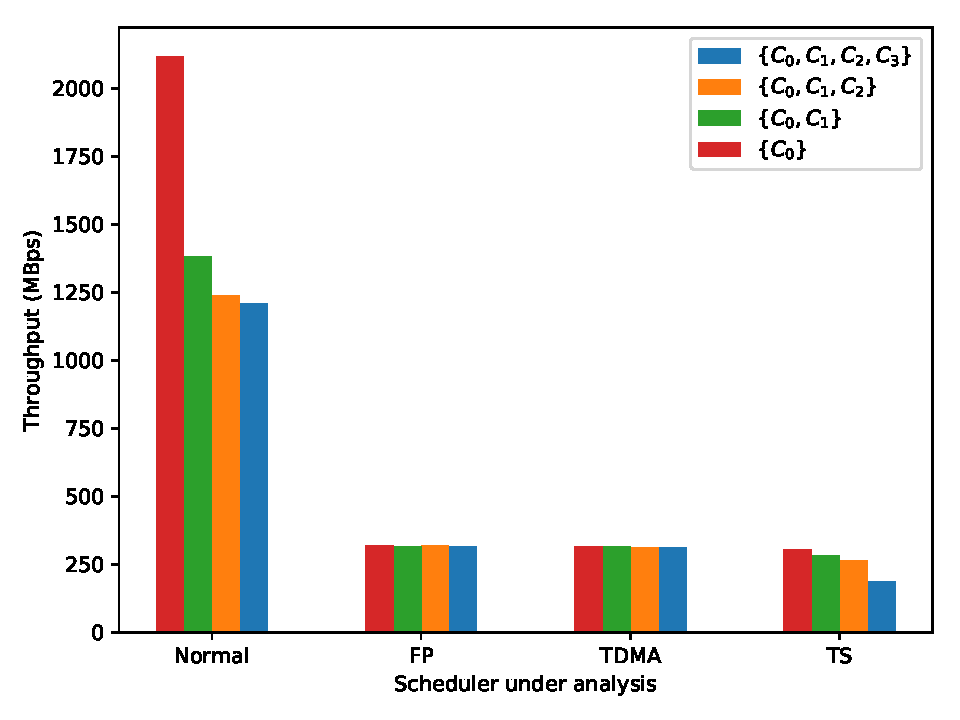
\includegraphics[scale=0.5]{images/bw_comparisons.pdf}
  \caption{Bandwidth in MBps for different path under increasing set of cores contending.}
  \label{fig:bandwidth_comparison}
\end{figure}

\subsection{Internal Behaviour of SchIM}
\label{subsec:internal-behaviour-of-schim}    
The next objective is to verify the correct behavior of our scheduling
policies at the granularity of a clock cycle by observing the inputs,
the outputs and the internal signals and registers of the \schim
module.  This is made possible thanks to the \emph{Integrated Logic
  Analyser} (or ILA) provided by Xilinx \cite{Xilinx-ILA}. The latter
IP can be directly implemented on the PL side, alongside the \schim,
and is able to probe the signals and to store them in a local
memory. For this experiment, a group of relevant internal signals have
been probed and captured during a window of 16384 contiguous clock
cycles. Then, the information has been extracted by post-processing
the data.  To characterize the behavior of the three different
policies, the ILA has been instrumented to collect (i) the amount of
transactions being buffered in the queues at each clock cycle (inset 1
in \fig{fig:schim_behaviour_fp}, \fig{fig:schim_behaviour_tdma}, and
\fig{fig:schim_behaviour_mg}), (ii) the rate at which queues receive
new transactions from the cores cluster (inset 2 in
\fig{fig:schim_behaviour_fp}, \fig{fig:schim_behaviour_tdma}, and
\fig{fig:schim_behaviour_mg}), and (iii) the queues ID of each
transaction forwarded by the \schim module (inset 3 in
\fig{fig:schim_behaviour_fp}, \fig{fig:schim_behaviour_tdma}, and
\fig{fig:schim_behaviour_mg}).
    
For the Fixed Priority trace snapshot displayed in
\fig{fig:schim_behaviour_fp}, the following strict priority ordering
has been considered: $C_{0} \succ C_{1} \succ C_{2} \succ C_{3}$ where
the $\succ$ operator means that the left argument has a strictly
higher priority than the right argument. In this experiment, a
regulation threshold of 2 for each core has been used.  As emphasized
by the inset 2 in \fig{fig:schim_behaviour_fp}, the FP scheduler is
able to prioritize the traffic of one core at the expense of the
others according to the priorities assignment. Furthermore, one can
observe that the rate at which the queues receive new transactions
from their associated core is proportional to the priority place in
the priority ordering.  Finally, the third inset in
\fig{fig:schim_behaviour_fp} confirms the correct behaviour of the FP
policy. Thanks to the heat map, one can clearly see that the cores
with the highest priority also feature the highest density of
transactions at the output of the \schim.
    
The trace snapshot displayed in \fig{fig:schim_behaviour_tdma} has
been obtained by configuring the \schim module in TDMA mode. For the
sake of clarity, a slot of 512 clock cycles have been set for each
core. In addition, the threshold of each core has been set to 1 to
create sharp transitions.  The insets 2 and 3 of
\fig{fig:schim_behaviour_tdma} clearly show the behaviour expected
from a TDMA schedule. In fact, one can clearly see in the latter that
transactions originating from one core are only being repeated out of
the \schim module during a well defined 512 clock cycles time
slot. Moreover, queues are scheduled one after the other in a periodic
fashion.  In the inset 2 of \fig{fig:schim_behaviour_tdma}, we can
observe a similar pattern, with transactions arriving only during the
TDMA slot associated to their queue (and indirectly core). Globally,
the rate at which queues receive transactions is steady and
constant. The variations can be explained by different factors such as
the coarseness of the FIQ feedback regulation and the scheduling
happening in the OS.
    
The trace snapshot for the TS policy has been obtained with the
minimal inter-arrival time set to 256 clock cycles for all the
cores. Similarly to the TDMA experiment, such period has been set
arbitrarily in order to improve the clarity of the trace snapshot
displayed in \fig{fig:schim_behaviour_mg}.  Thanks to the inset 3 in
\fig{fig:schim_behaviour_mg}, we can see that under a significant
traffic load, the TS mode of the \schim is able to shape the output
traffic. Roughly, the same pattern can be observed in inset 2 of
\fig{fig:schim_behaviour_mg}. However, there are two
exceptions. First, one queue can receive more than one
transaction. This is due to the coarseness of the FIQ feedback
regulation. Secondly, some queues seem to be prioritized. This can be
explained by the fact that in the TS scheduler implementation break
ties between valid ready transactions using a FP policy. In this
experiment, since the \schim module is constantly under pressure,
there are always ties between the queues and FP is frequently applied.
    \begin{figure}[]
      \centering
      \begin{subfigure}{0.5\textwidth}
        \centering
        % include first image
        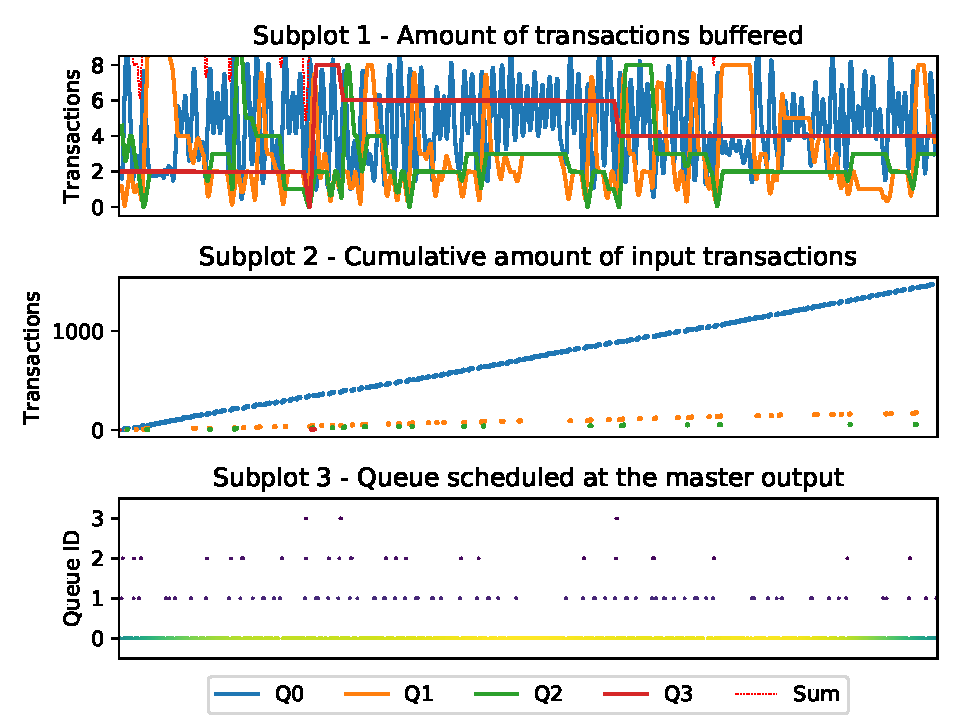
\includegraphics[scale=0.55]{images/SchIM_FP_buffering.pdf}
        \caption{FP with ordering $C_{0} \succ C_{1} \succ C_{2} \succ C_{3}$}
        \label{fig:schim_behaviour_fp}
      \end{subfigure}
      \vfill
      \begin{subfigure}{0.5\textwidth}
        \centering
        % include second image
        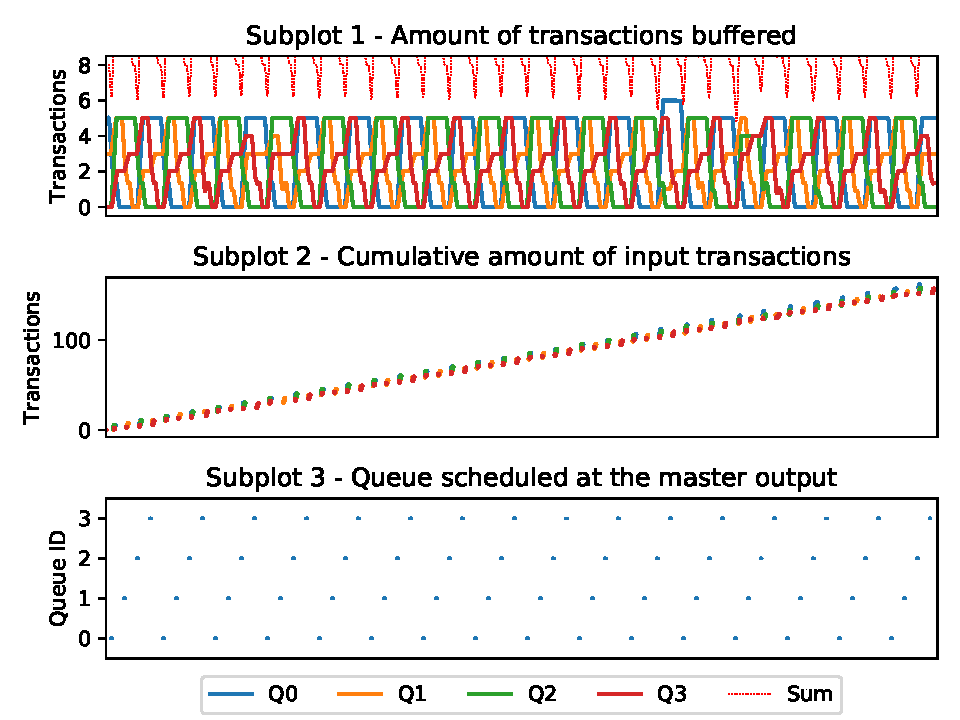
\includegraphics[scale=0.55]{images/SchIM_TDMA_buffering.pdf}
        \caption{TDMA with slots of 512 clock cycles}
        \label{fig:schim_behaviour_tdma}
      \end{subfigure}
      \vfill
      \begin{subfigure}{0.5\textwidth}
        \centering
        % include second image
        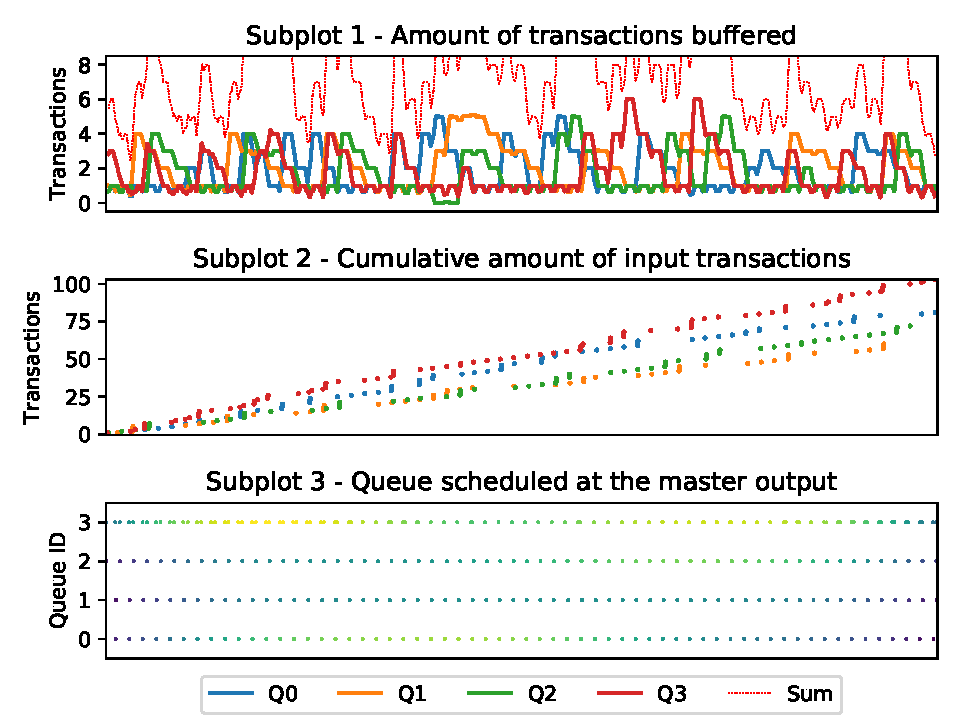
\includegraphics[scale=0.55]{images/SchIM_MG_buffering.pdf}
        \caption{TS with min. period of 256 clock cycles}
        \label{fig:schim_behaviour_mg}
      \end{subfigure}
      \caption{Trace snapshots of SchIM for FP (\ref{fig:schim_behaviour_fp}), TDMA (\ref{fig:schim_behaviour_tdma}) and TS (\ref{fig:schim_behaviour_mg})}
      \label{fig:schim_behaviour}
    \end{figure}

\subsection{Memory Isolation}\label{subsec:isolation}
To evaluate the capability of \schim with respect to its ability to
ensure performance isolation between the cores, a set of experiments
involving SD-VBS benchmarks were designed. Here, we compare the
execution time of an application on a given core when running
alongside interfering synthetic benchmarks (memory bombs) on all the
other cores. The slowdown compared to the case in which the observed
benchmark runs alone in the system is computed. It follows that a
ratio of 1 denotes the ideal isolation. The results obtained on the
considered benchmarks are listed in
Table~\ref{tab:isolation_ratio}. All the results in the table are the
aggregation (geometric average) of 100 different runs in the same
configuration.

The simple loop-back path is used as a baseline for this experiment
because scheduling is performed in this configuration. The results for
the simple loop-back are displayed in the left-most column in
Table~\ref{tab:isolation_ratio}. We highlight the sensitivity of both
\emph{disparity} and \emph{mser} to inter-core interference, with
ratios of respectively $1.46$ and $1.59$. On the other hand,
\emph{texture synthesis} and \emph{localization} do not seem to suffer
significantly from inter-core interference. In comparison, the TDMA
scheduler manages to guarantee isolation of the core under
analysis. In fact, the ratio of all the benchmarks we tested lie in
the proximity of 1.0, with a maximum inter-core interference of around
7\%. Similarly, the TS scheduler is also capable of ensuring a sound
isolation of the core under analysis. Unfortunately, the FP scheduler
is unable to guarantee the isolation of the core under analysis
despite having been assigned the highest priority. Even worst, the
scheduler has little-to-none impact since its slowdown is comparable
to that observed on the loop-back path.  This result can be explained
by the fact that, despite the enforcement of the FP policy, and its
proven correct behaviour (see \fig{fig:schim_behaviour_fp}), the
enforced ordering of transaction is likely overridden by the
transaction re-ordering mechanisms present in the DDR controller. The
problem specifically occurs because the access pattern of the
interfering bombs is sequential, and hence preferably treated by the
DDR controller. Conversely, the FP scheduler works correctly in
scenarios like those in \fig{fig:schim_behaviour_fp} because the
memory access pattern of the core under analysis is sequential as
well. It follows that the FP policy is mainly useful when performing
the movement of large, sequential data chunks.
\begin{table}[]
  \centering
  \caption{Inter-core Interference Ratios}
  \label{tab:isolation_ratio}
  \begin{tabular}{|l||c|c|c|c|}
    \hline
    \multirow{2}{*}{Benchmark} & \multicolumn{4}{c|}{Memory Route \& Scheduler}                          \\ \cline{2-5} 
    & Loop-back & \schim TDMA & \schim TS & \schim FP \\ \hline\hline
    stitch                     & $1.14$    & $1.06$      & $0.98$    & $1.16$    \\ \hline
    texture synth.             & $1.03$    & $1.02$      & $1.0$     & $1.03$    \\ \hline
    disparity                  & $1.46$    & $1.07$      & $0.96$    & $1.46$    \\ \hline
    tracking                   & $1.13$    & $1.05$      & $0.97$    & $1.13$    \\ \hline
    localization               & $1.02$    & $1.01$      & $1.0$     & $1.02$    \\ \hline
    mser                       & $1.59$    & $1.06$      & $0.98$    & $1.56$    \\ \hline
    sift                       & $1.14$    & $1.04$      & $0.97$    & $1.14$    \\ \hline
  \end{tabular}
\end{table}
